\subsubsection{End-to-end feature-discovery comparison on session B}
\label{subsubsection:rebuttal_discovery_comparison}

We compare NLDisco with CEBRA-Time, LangevinFlow, ST-NDT, and PCA on feature discovery from start to finish on session B, a second 18-hour recording from the same mouse and probe insertion as the recording of Section~\ref{subsection:aeon_results} (session A), taken one day earlier (June 5, 2024, 23:00 to June 6, 17:00), spike-sorted separately and prepared in the same way: every method is fitted to the neural activity of one part of the recording, latents are inspected and interpreted on that part, and each interpretation is tested on a held-out part. Part A asks how many behavioral features defined in advance each method recovers. Part B asks what share of randomly drawn latents receives an interpretation, from raters who do not know which method a latent comes from, that holds on the held-out part. All methods share the split, the inspection budget, the interpretation criterion, and the held-out test. The split, the methods and their candidate settings, the scoring rule, the pass criteria, the Part A feature definitions, and the Part B sampling and validation rules were fixed before the session B data were prepared; the ST-NDT settings were added before any ST-NDT run. The code was developed on session A only, and the rater instructions were finalized on practice cards from session A before any rater saw a session B card.

\paragraph{Data and split.}
Session B has 87 units and 3,238,618 valid 0.4-s windows ($S=20$ bins of 20 ms); a window is assigned the behavior at its last bin. The recording is cut into 20 equal blocks of time. Blocks 4, 8, 12, 16, and 20 form the held-out part (809,575 windows), and the other 15 blocks form the discovery part. Within each discovery block, the first 90\% is the fit portion (2,185,752 windows) and the last 10\% the validation portion (242,664 windows); the 627 windows that span two portions are dropped. Models are fitted on the fit portion without behavior. The validation portion serves only to choose between candidate settings of a baseline by that baseline's own loss. Latent selection, activation thresholds, and the material shown to raters use the discovery part, and the held-out part is used only for scoring.

\paragraph{Methods.}
NLDisco is the TW-SED of Section~\ref{subsection:aeon_results} ($S=20$, $(D_1,k_1)=(96,6)$, $(D_2,k_2)=(192,12)$, $B=1024$, 5,000 updates), trained once with no selection between runs. CEBRA-Time and LangevinFlow follow the configurations of Section~\ref{subsection:churchland_results} with their encoders extended to 20-bin windows, and are trained for 5,000 updates of 1,024 windows. For CEBRA-Time (temperature 1, positive-pair lag of one bin, 128 hidden units) we compare learning rates $10^{-4}$, $3\times10^{-4}$, and $10^{-3}$ and select $10^{-3}$ (validation InfoNCE loss $5.955$, against $5.961$ and $5.973$). For LangevinFlow (64-dimensional position, momentum, and recurrent states, concatenated to 192 latents) we compare learning rates $\{0.001, 0.003\}$ and regularization-ramp durations $\{5, 500\}$ and select $0.001$ and $500$ (validation masked Poisson negative log-likelihood $0.2864$, against $0.2868$--$0.2980$). ST-NDT~\citep{le_2022_stndt}, a spatiotemporal Transformer trained with masked spike prediction and a contrastive loss, is run from its published implementation on the same windows; we compare contrastive-loss weights $\{0.01, 0.1, 1\}$ at learning rate $0.001$ and learning rate $0.003$ at weight $0.1$, and select weight $0.1$ with learning rate $0.003$ (validation masked Poisson negative log-likelihood $0.3397$, against $0.3398$--$0.3451$). ST-NDT is trained in whole epochs, here three epochs of the fit portion (6,405 updates of 1,024 windows), and its width is tied to the number of units, so it provides 87 latents. PCA takes the first 192 principal components of the standardized, flattened 20-bin window. No setting is chosen using behavior, and each method is run with one seed. Every method yields one vector per window, and each of its coordinates is a candidate latent: 192 for NLDisco, CEBRA-Time, LangevinFlow, and PCA, and 87 for ST-NDT.

\paragraph{Scoring rule and interpretation criterion.}
One rule scores a latent against a behavioral condition for every method and in both parts. The latent is given a direction, high or low, and its values are sign-reversed for low. Its activation threshold is the value that maximizes $\metric{Cov}+\metric{Spec}-1$ on the discovery part, and the latent is active when its value is at or above this threshold. With this direction and threshold, \metric{Cov}, \metric{Spec}, \metric{Sel}, and \metric{AUROC} (\hyperref[subsubsection:latents_evaluation_details]{\ref*{subsubsection:latents_evaluation_details}}) are computed on the held-out part. An interpretation passes if its held-out \metric{AUROC} and \metric{Sel} are both at least $0.75$. Three alternative criteria were fixed at the same time: both at least $0.70$, both at least $0.80$, and \metric{AUROC} alone at least $0.75$.

\paragraph{Part A: prespecified features.}
We defined 23 features from the behavior variables alone, covering position, speed, acceleration, movement direction, movement relative to the patch, body area, wheel running, and food delivery (\autoref{table:rebuttal_discovery_definitions}). For each method and feature, every latent is oriented so that its discovery-part \metric{AUROC} is at least $0.5$, the latent with the highest discovery-part \metric{AUROC} is selected, and the scoring rule is applied. A feature is recovered if the selected latent passes the criterion on the held-out part.

ST-NDT recovers 12 of the 23 features, NLDisco 10, PCA 9, CEBRA-Time 5, and LangevinFlow 2 (\autoref{table:rebuttal_discovery_part_a_summary}; per-feature scores in \autoref{table:rebuttal_discovery_part_a_scores}). NLDisco recovers \textit{at the most occupied location}, \textit{moving}, \textit{fast locomotion}, \textit{accelerating}, \textit{decelerating}, \textit{wheel running}, \textit{wheel-bout onset}, \textit{wheel-bout offset}, \textit{after a pellet trigger}, and \textit{before a pellet trigger}. ST-NDT recovers the same ten features and, in addition, \textit{stationary} (\metric{AUROC} $0.81$, \metric{Sel} $0.78$; NLDisco $0.75$, $0.70$) and \textit{small body area} ($0.75$, $0.77$; NLDisco $0.73$, $0.71$). PCA recovers NLDisco's ten features except \textit{after a pellet trigger}. CEBRA-Time recovers the three wheel features and the two pellet features, and has the highest scores of any method on the wheel features and on \textit{before a pellet trigger} (\metric{AUROC} $0.91$--$0.95$). LangevinFlow recovers \textit{at the most occupied location} and \textit{fast locomotion}. No method recovers the four movement-direction features, the two features of movement relative to the patch, \textit{near the patch}, \textit{elsewhere in the arena}, \textit{large body area}, \textit{fast wheel running}, or \textit{at the patch, wheel idle}. Under the alternative criteria, the counts are 12 for ST-NDT and NLDisco, 11 for PCA, 7 for LangevinFlow, and 6 for CEBRA-Time (both scores at least $0.70$); 5 for NLDisco and PCA, 4 for CEBRA-Time, 3 for ST-NDT, and 0 for LangevinFlow (both at least $0.80$); and 14 for ST-NDT and PCA, 11 for NLDisco, 8 for LangevinFlow, and 7 for CEBRA-Time (\metric{AUROC} alone).

\begin{table}[!htbp]
    \centering
    {\small\setlength{\tabcolsep}{3pt}\renewcommand{\arraystretch}{1.1}
    \begin{tabular*}{\linewidth}{@{\extracolsep{\fill}}lrrrrrrrrr@{}}
\toprule
Method & Latents & Recovered & \shortstack{Both\\$\geq0.70$} & \shortstack{Both\\$\geq0.80$} & \shortstack{\metric{AUROC}\\$\geq0.75$} & \metric{Cov} & \metric{Spec} & \metric{Sel} & \metric{AUROC} \\
\midrule
NLDisco & 192 & 10/23 & 12 & 5 & 11 & 0.72 & 0.70 & 0.71 & 0.74 \\
CEBRA-Time & 192 & 5/23 & 6 & 4 & 7 & 0.66 & 0.68 & 0.68 & 0.72 \\
LangevinFlow & 192 & 2/23 & 7 & 0 & 8 & 0.67 & 0.62 & 0.64 & 0.68 \\
ST-NDT & 87 & \textbf{12}/23 & 12 & 3 & 14 & 0.73 & 0.68 & 0.70 & 0.76 \\
PCA & 192 & 9/23 & 11 & 5 & 14 & 0.72 & 0.70 & 0.70 & 0.76 \\
\bottomrule
\end{tabular*}
}
    \caption{\textbf{Part A: recovery of 23 prespecified behavioral features on the held-out part of session B.} ``Recovered'' counts features whose selected latent has held-out \metric{AUROC} $\geq0.75$ and \metric{Sel} $\geq0.75$; the highest count is in bold. The next three columns give the counts under the alternative criteria (``Both'': \metric{AUROC} and \metric{Sel}). \metric{Cov}, \metric{Spec}, \metric{Sel}, and \metric{AUROC} are held-out means over the 23 features. ``Latents'' is the number of candidate latents of each method.}
    \label{table:rebuttal_discovery_part_a_summary}
\end{table}

\begin{table}[!htbp]
    \centering
    {\footnotesize\setlength{\tabcolsep}{2pt}\renewcommand{\arraystretch}{1.05}
    \begin{tabular*}{\linewidth}{@{\extracolsep{\fill}}rp{0.19\linewidth}p{0.36\linewidth}p{0.24\linewidth}r@{}}
\toprule
\# & Feature & Condition & Compared within & \%  \\
\midrule
1 & near the patch & patch distance $\leq$ 100 px & valid tracking & 13.3 \\
2 & moving & speed $\geq$ 20 px/s & valid tracking & 12.4 \\
3 & accelerating & acceleration $\geq$ 200 px/s$^2$ & valid tracking & 3.0 \\
4 & decelerating & acceleration $\leq-200$ px/s$^2$ & valid tracking & 3.2 \\
5 & moving right ($+x$) & movement direction within 45$^\circ$ of $+x$ & valid tracking, speed $\geq$ 20 px/s & 25.4 \\
6 & moving down ($+y$) & movement direction within 45$^\circ$ of $+y$ & valid tracking, speed $\geq$ 20 px/s & 24.4 \\
7 & moving left ($-x$) & movement direction within 45$^\circ$ of $-x$ & valid tracking, speed $\geq$ 20 px/s & 27.0 \\
8 & moving up ($-y$) & movement direction within 45$^\circ$ of $-y$ & valid tracking, speed $\geq$ 20 px/s & 23.2 \\
9 & moving toward the patch & movement direction within 45$^\circ$ of the direction to the patch & valid tracking, speed $\geq$ 20 px/s & 21.5 \\
10 & wheel spinning & wheel speed $>$ 0.05 turns/s & valid wheel samples & 2.5 \\
11 & fast wheel spinning & wheel speed $\geq$ median wheel speed of wheel-spinning windows in the discovery part (0.309 turns/s) & wheel-spinning windows & 53.4 \\
12 & wheel-bout onset & 0 to 0.5 s after a wheel bout starts & valid wheel samples & 0.8 \\
\bottomrule
\end{tabular*}
}
    \caption{\textbf{Part A feature definitions.} Each feature is a condition on the behavior at the last bin of a window, compared against all other windows of the stated set; a window enters only if its whole 20-bin span has valid samples of the variables involved. Quantiles and the most occupied location are computed on the discovery part. A wheel bout is wheel speed above $0.05$ turns/s, with pauses shorter than $0.2$ s filled and bouts shorter than $0.4$ s removed. ``\%'' is the share of compared held-out windows in which the condition holds.}
    \label{table:rebuttal_discovery_definitions}
\end{table}

\begin{table}[!htbp]
    \centering
    {\scriptsize\setlength{\tabcolsep}{2pt}\renewcommand{\arraystretch}{1.1}
    \begin{tabular*}{\linewidth}{@{\extracolsep{\fill}}rlrrrrrrrrrr@{}}
\toprule
 & & \multicolumn{2}{c}{NLDisco} & \multicolumn{2}{c}{CEBRA-Time} & \multicolumn{2}{c}{LangevinFlow} & \multicolumn{2}{c}{ST-NDT} & \multicolumn{2}{c}{PCA} \\
\# & Feature & \metric{AUROC} & \metric{Sel} & \metric{AUROC} & \metric{Sel} & \metric{AUROC} & \metric{Sel} & \metric{AUROC} & \metric{Sel} & \metric{AUROC} & \metric{Sel} \\
\midrule
1 & near the patch & 0.65 & 0.59 & 0.67 & 0.60 & 0.62 & 0.58 & 0.79 & 0.64 & 0.75 & 0.66 \\
2 & at the most occupied location & \textbf{0.76} & \textbf{0.79} & 0.68 & 0.68 & \textbf{0.77} & \textbf{0.77} & \textbf{0.85} & \textbf{0.88} & \textbf{0.84} & \textbf{0.85} \\
3 & elsewhere in the arena & 0.74 & 0.66 & 0.66 & 0.59 & 0.77 & 0.67 & 0.78 & 0.63 & 0.81 & 0.68 \\
4 & stationary & 0.75 & 0.70 & 0.68 & 0.65 & 0.77 & 0.71 & \textbf{0.81} & \textbf{0.78} & 0.81 & 0.74 \\
5 & moving & \textbf{0.86} & \textbf{0.79} & 0.75 & 0.68 & 0.85 & 0.74 & \textbf{0.90} & \textbf{0.80} & \textbf{0.91} & \textbf{0.83} \\
6 & fast locomotion & \textbf{0.93} & \textbf{0.82} & 0.82 & 0.72 & \textbf{0.86} & \textbf{0.75} & \textbf{0.94} & \textbf{0.85} & \textbf{0.93} & \textbf{0.85} \\
7 & accelerating & \textbf{0.85} & \textbf{0.77} & 0.74 & 0.67 & 0.85 & 0.74 & \textbf{0.89} & \textbf{0.79} & \textbf{0.88} & \textbf{0.79} \\
8 & decelerating & \textbf{0.85} & \textbf{0.76} & 0.76 & 0.68 & 0.80 & 0.70 & \textbf{0.87} & \textbf{0.76} & \textbf{0.89} & \textbf{0.80} \\
9 & moving right ($+x$) & 0.52 & 0.51 & 0.58 & 0.61 & 0.53 & 0.52 & 0.59 & 0.58 & 0.56 & 0.55 \\
10 & moving down ($+y$) & 0.53 & 0.53 & 0.58 & 0.57 & 0.56 & 0.54 & 0.56 & 0.57 & 0.55 & 0.55 \\
11 & moving left ($-x$) & 0.60 & 0.59 & 0.55 & 0.54 & 0.53 & 0.52 & 0.58 & 0.55 & 0.58 & 0.57 \\
12 & moving up ($-y$) & 0.55 & 0.73 & 0.58 & 0.60 & 0.54 & 0.54 & 0.59 & 0.57 & 0.55 & 0.56 \\
13 & moving toward the patch & 0.56 & 0.54 & 0.60 & 0.59 & 0.55 & 0.53 & 0.60 & 0.57 & 0.61 & 0.60 \\
14 & moving away from the patch & 0.65 & 0.65 & 0.65 & 0.60 & 0.56 & 0.54 & 0.61 & 0.57 & 0.66 & 0.62 \\
15 & small body area & 0.73 & 0.71 & 0.69 & 0.67 & 0.77 & 0.67 & \textbf{0.75} & \textbf{0.77} & 0.76 & 0.70 \\
16 & large body area & 0.64 & 0.71 & 0.59 & 0.57 & 0.60 & 0.62 & 0.67 & 0.69 & 0.68 & 0.68 \\
17 & wheel running & \textbf{0.90} & \textbf{0.82} & \textbf{0.93} & \textbf{0.90} & 0.71 & 0.72 & \textbf{0.88} & \textbf{0.78} & \textbf{0.87} & \textbf{0.77} \\
18 & fast wheel running & 0.64 & 0.62 & 0.64 & 0.58 & 0.57 & 0.54 & 0.61 & 0.57 & 0.61 & 0.56 \\
19 & wheel-bout onset & \textbf{0.93} & \textbf{0.87} & \textbf{0.95} & \textbf{0.92} & 0.74 & 0.75 & \textbf{0.89} & \textbf{0.78} & \textbf{0.91} & \textbf{0.84} \\
20 & wheel-bout offset & \textbf{0.90} & \textbf{0.85} & \textbf{0.93} & \textbf{0.91} & 0.71 & 0.63 & \textbf{0.87} & \textbf{0.76} & \textbf{0.90} & \textbf{0.82} \\
21 & at the patch, wheel idle & 0.69 & 0.62 & 0.70 & 0.64 & 0.67 & 0.59 & 0.73 & 0.63 & 0.70 & 0.61 \\
22 & after a pellet trigger & \textbf{0.90} & \textbf{0.81} & \textbf{0.82} & \textbf{0.78} & 0.74 & 0.65 & \textbf{0.90} & \textbf{0.85} & 0.81 & 0.68 \\
23 & before a pellet trigger & \textbf{0.83} & \textbf{0.76} & \textbf{0.91} & \textbf{0.87} & 0.68 & 0.63 & \textbf{0.87} & \textbf{0.76} & \textbf{0.87} & \textbf{0.79} \\
\midrule
\multicolumn{2}{l}{Features recovered} & \multicolumn{2}{c}{10} & \multicolumn{2}{c}{5} & \multicolumn{2}{c}{2} & \multicolumn{2}{c}{12} & \multicolumn{2}{c}{9} \\
\bottomrule
\end{tabular*}
}
    \caption{\textbf{Part A held-out scores per feature.} Held-out \metric{AUROC} and \metric{Sel} of the latent selected for each feature on the discovery part. Bold marks recovered features (both scores $\geq0.75$). Features are numbered as in \autoref{table:rebuttal_discovery_definitions}.}
    \label{table:rebuttal_discovery_part_a_scores}
\end{table}

\paragraph{Part B: blind discovery.}
From each method we draw 32 latents uniformly at random, without replacement and with a fixed seed, from the latents that are not constant on the discovery part; the same 160 latents go to every rater. For each latent, the same code builds one text card from the discovery part only. A card gives percentiles of the latent's values, the definition of its high state (every value above its minimum if the latent sits at its minimum in at least half of the windows, and the top 5\% of values otherwise, in which case the bottom 5\% defines a low state), the number and duration of high episodes and their share in each block of the recording, a tuning table for every behavior variable (share of windows, mean rank of the latent's value, and share of high and low windows per bin), a position map, and the behavior at a few example episodes. Cards carry a random identifier and neither the method nor the latent index.

The raters are three AI agents (Claude Sonnet 5.5 at high reasoning effort). Each is a separate, fresh agent that receives the same written instructions, which state that the latents come from several models, are shown in random order, and are not labelled by model. A rater sees one card at a time through a command-line tool, in its own random order arranged in rounds of one card per method, cannot revisit a card, and has no access to the other raters' answers, to the models, to the assignment of cards to methods, or to the held-out part. For each card the rater answers either ``no interpretation'' or one rule with a direction (the latent is high, or low, when the rule holds). A rule is a Boolean expression on the behavior variables (position $x$ and $y$, distance to the patch, speed, acceleration, movement direction, movement direction relative to the patch, velocity toward the patch, body area, wheel speed, time since the last pellet trigger, and time to the next), built from comparisons, \texttt{and}, \texttt{or}, \texttt{not}, arithmetic, and the functions \texttt{abs} and \texttt{hypot}. The instructions describe the pass criterion and state that a rule that fails counts against the rater as much as a missed interpretation.

A rule is evaluated on all held-out windows with valid samples of its variables and scored with the scoring rule above, using the rater's direction. The interpretation is validated if it passes the criterion (held-out \metric{AUROC} and \metric{Sel} both at least $0.75$) and the rule holds in at least 500 and fails in at least 500 held-out windows. To count distinct features, the validated rules of all methods and raters are clustered by the absolute correlation of their held-out condition masks (average linkage, cut at $0.5$), and a method surfaces a feature if at least one of its validated rules lies in the cluster.

The share of inspected latents with a validated interpretation, averaged over the three raters, is 90\% for ST-NDT, 63\% for LangevinFlow, 29\% for CEBRA-Time, 8\% for NLDisco, and 6\% for PCA (\autoref{table:rebuttal_discovery_part_b_summary}). The raters agree closely: Fleiss' $\kappa$ over the 160 cards is $0.94$ for whether a latent has a validated interpretation and $0.92$ for whether a rule was given. Raters spent about 5 s per card for every method ($4.7$--$5.4$ s), so a validated interpretation costs $1.1$ inspected latents for ST-NDT, $1.6$ for LangevinFlow, $3.4$ for CEBRA-Time, $12$ for NLDisco, and $16$ for PCA. Of the 32 sampled NLDisco latents, 29 received no interpretation from any rater; 22 of these are active in fewer than $0.2\%$ of windows.

The validated rules form six distinct features (\autoref{table:rebuttal_discovery_part_b_features}). ST-NDT and CEBRA-Time each surface five, NLDisco three, and LangevinFlow and PCA two. All five methods surface the first $0.5$ s after a pellet trigger. NLDisco also surfaces wheel running in the seconds before a pellet trigger and a place field at the edge of the arena, both of which ST-NDT and CEBRA-Time surface as well. Small body area is surfaced by CEBRA-Time and ST-NDT, the interval $0.5$--$1$ s after a pellet trigger by CEBRA-Time and LangevinFlow, and fast movement by ST-NDT alone. The two features in the first second after a pellet trigger account for 47 of the 66 latents validated by at least one rater (20 of 20 for LangevinFlow, 20 of 29 for ST-NDT, 5 of 12 for CEBRA-Time, 1 of 3 for NLDisco, and 1 of 2 for PCA). In a comparison that was not prespecified, the validated interpretations of NLDisco latents have the highest held-out selectivity, with a median \metric{Sel} over validated rules of $0.98$ against $0.92$ for LangevinFlow, $0.88$ for ST-NDT and PCA, and $0.83$ for CEBRA-Time. \autoref{fig:rebuttal_discovery_examples} shows, for each method, the validated interpretation with the highest held-out \metric{AUROC}.

\begin{table}[!htbp]
    \centering
    {\footnotesize\setlength{\tabcolsep}{2pt}\renewcommand{\arraystretch}{1.1}
    \begin{tabular*}{\linewidth}{@{\extracolsep{\fill}}lrrrrrrrrr@{}}
\toprule
Method & \shortstack{Latents\\inspected} & \shortstack{Given a\\rule} & \shortstack{Validated\\(range)} & \shortstack{Validated\\share} & \shortstack{Validated,\\$\geq2$ raters} & \shortstack{Fleiss'\\$\kappa$} & \shortstack{Distinct\\features} & \shortstack{Latents\\per\\validated} & \shortstack{Rater\\min per\\validated} \\
\midrule
NLDisco & 32 & 3.0 & 2.7 (2--3) & 8\% & 3 & 0.86 & 3 & 12.0 & 1.0 \\
CEBRA-Time & 32 & 11.7 & 9.3 (7--11) & 29\% & 9 & 0.75 & 5 & 3.4 & 0.3 \\
LangevinFlow & 32 & 21.3 & 20.0 (20--20) & 63\% & 20 & 1.00 & 2 & 1.6 & 0.1 \\
ST-NDT & 32 & 30.7 & 28.7 (28--29) & \textbf{90\%} & 29 & 0.89 & 5 & 1.1 & 0.1 \\
PCA & 32 & 2.3 & 2.0 (2--2) & 6\% & 2 & 1.00 & 2 & 16.0 & 1.2 \\
\bottomrule
\end{tabular*}
}
    \caption{\textbf{Part B: blind discovery on 32 random latents per method.} ``Given a rule'' and ``Validated'' are numbers of latents, averaged over the three raters, with the range over raters in parentheses. ``Validated share'' is the mean number validated divided by 32; the highest share is in bold. ``Validated, $\geq2$ raters'' counts latents with a validated interpretation from at least two raters. Fleiss' $\kappa$ is for whether a latent has a validated interpretation. ``Latents per validated'' is the number of latents inspected per validated interpretation, and ``Rater min per validated'' the corresponding rater time in minutes, measured from showing a card to receiving its answer.}
    \label{table:rebuttal_discovery_part_b_summary}
\end{table}

\begin{table}[!htbp]
    \centering
    {\footnotesize\setlength{\tabcolsep}{3pt}\renewcommand{\arraystretch}{1.1}
    \begin{tabular*}{\linewidth}{@{\extracolsep{\fill}}rp{0.42\linewidth}ccccc@{}}
\toprule
\# & Representative rule (direction) & NLDisco & CEBRA-Time & LangevinFlow & ST-NDT & PCA \\
\midrule
1 & \texttt{time\_since\_pellet $\leq$ 0.5} (low) & \checkmark & \checkmark & \checkmark & \checkmark & \checkmark \\
2 & \texttt{time\_to\_pellet $\leq$ 5} (low) & \checkmark & \checkmark &  & \checkmark & \checkmark \\
3 & \texttt{x $\geq$ 1200 and y $\geq$ 400 and y $<$ 600} (high) & \checkmark & \checkmark &  & \checkmark &  \\
4 & \texttt{time\_since\_pellet $\geq$ 0.5 and time\_since\_pellet $\leq$ 1} (high) &  & \checkmark & \checkmark &  &  \\
5 & \texttt{area $<$ 342} (high) &  & \checkmark &  & \checkmark &  \\
6 & \texttt{speed $\geq$ 100} (low) &  &  &  & \checkmark &  \\
\bottomrule
\end{tabular*}
}
    \caption{\textbf{Distinct features surfaced in Part B.} Each row is one cluster of validated rules, shown by a representative rule in the raters' rule language and the direction of the latent when the rule holds. Times are in seconds, positions in px, area in px$^2$, and speed in px/s. A check mark means that at least one validated rule of the method lies in the cluster.}
    \label{table:rebuttal_discovery_part_b_features}
\end{table}

\begin{figure}[!htbp]
    \centering
    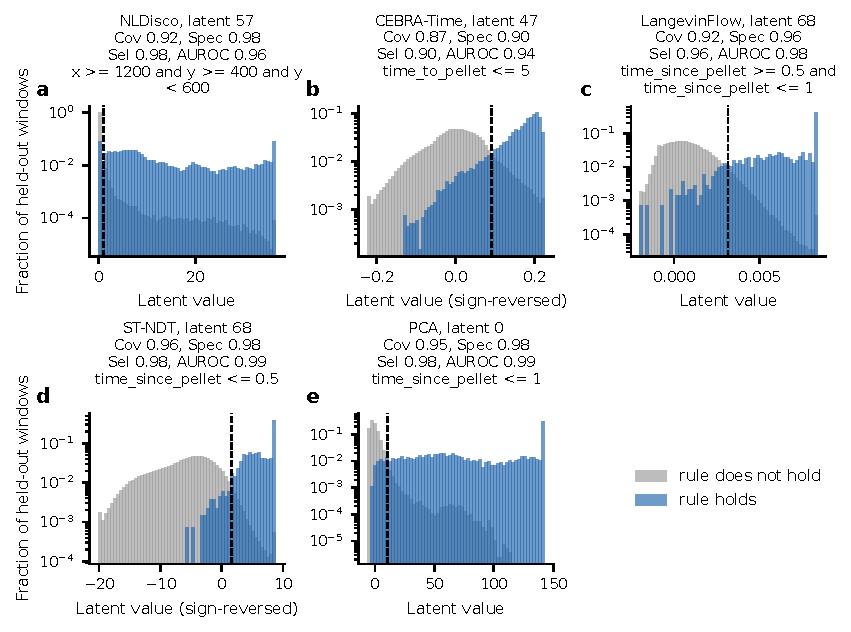
\includegraphics[width=\linewidth]{figures/rebuttal/change03_discovery/examples.pdf}
    \caption{\textbf{One validated interpretation per method.} For each method, the validated Part B interpretation with the highest held-out \metric{AUROC}: distributions of the latent's value over held-out windows in which the rater's rule holds and in which it does not (log scale), with the rule and held-out scores above each panel. Values are sign-reversed where the rater's direction is low. Dashed line: activation threshold fitted on the discovery part.}
    \label{fig:rebuttal_discovery_examples}
\end{figure}

\paragraph{Post hoc variant: excluding the second after each pellet trigger.}
This variant was defined after the results above had been seen. Because most validated Part B interpretations concern the first second after a pellet trigger, we examined the population activity around the triggers. In session B, the summed spike count of the 87 units rises from 16 spikes per 20-ms bin before a trigger to a mean of 104 over the first $0.26$ s after it, about a sixfold increase, stays between three and four times the earlier level until $0.62$ s, and falls back within 80 ms. The rise follows 175 of the 176 triggers, and we did not determine its source. In the variant, all windows that end less than 1 s after a pellet trigger are removed from latent selection, threshold fitting, and held-out scoring in both parts. The models and the raters' answers are those of the main analysis, so the raters' cards included these windows.

In the variant, ST-NDT recovers 12 of the 23 Part A features, NLDisco 10, PCA 10, CEBRA-Time 4, and LangevinFlow 2 (\autoref{table:rebuttal_discovery_posthoc}). In Part B, the share of inspected latents with a validated interpretation is 33\% for ST-NDT, 16\% for CEBRA-Time, 6\% for NLDisco, 2\% for PCA, and 0\% for LangevinFlow, with Fleiss' $\kappa=0.82$. The validated rules form four distinct features: the place field (NLDisco, CEBRA-Time, and ST-NDT), wheel running before a pellet trigger (NLDisco, CEBRA-Time, ST-NDT, and PCA), small body area (CEBRA-Time and ST-NDT), and fast movement (ST-NDT).

\begin{table}[!htbp]
    \centering
    {\small\setlength{\tabcolsep}{3pt}\renewcommand{\arraystretch}{1.1}
    \begin{tabular*}{\linewidth}{@{\extracolsep{\fill}}lrrrrrr@{}}
\toprule
 & \multicolumn{2}{c}{Part A: recovered} & \multicolumn{4}{c}{Part B: validated interpretations} \\
\cmidrule(lr){2-3}\cmidrule(l){4-7}
Method & \shortstack{All\\windows} & \shortstack{Post hoc\\variant} & \shortstack{Share, all\\windows} & \shortstack{Share, post\\hoc variant} & \shortstack{Latents, post hoc\\variant (range)} & \shortstack{Distinct features,\\post hoc variant} \\
\midrule
NLDisco & 10/23 & 10/23 & 8\% & 6\% & 2.0 (2--2) & 2 \\
CEBRA-Time & 5/23 & 4/23 & 29\% & 16\% & 5.0 (3--7) & 3 \\
LangevinFlow & 2/23 & 2/23 & 63\% & 0\% & 0.0 (0--0) & 0 \\
ST-NDT & 12/23 & 12/23 & 90\% & 33\% & 10.7 (10--12) & 4 \\
PCA & 9/23 & 10/23 & 6\% & 2\% & 0.7 (0--1) & 1 \\
\bottomrule
\end{tabular*}
}
    \caption{\textbf{Post hoc variant without the second after each pellet trigger.} Part A counts of recovered features and Part B validated interpretations with all windows (\autoref{table:rebuttal_discovery_part_a_summary} and \autoref{table:rebuttal_discovery_part_b_summary}) and in the variant, which removes windows ending less than 1 s after a pellet trigger from latent selection, threshold fitting, and held-out scoring. ``Latents'' is the number of validated latents of 32, averaged over raters, with the range over raters in parentheses. The variant was defined after the all-window results had been seen.}
    \label{table:rebuttal_discovery_posthoc}
\end{table}
